\documentclass[a4paper]{article}
\usepackage{xcolor}
\usepackage[colorlinks=false, urlcolor=black, linkcolor=black, linkbordercolor=black]{hyperref}

\usepackage{amsmath}
\usepackage{amsthm}
\usepackage{amssymb}
\usepackage{cases}

\usepackage{tikz}

\usepackage{hyperref}

\usepackage[margin=1.5cm]{geometry}
\usetikzlibrary{matrix}

\begin{document}
\title{\textbf{On a Property of Magic Squares}}
\author{Gavin A. Forrester}
\maketitle

\section*{Preface}
This is a submission to the The Summer of Math Exposition (SoME), summer 2025. The paper demonstrates a simple concept that is new and what happens when it is in the format of a formal mathematics paper.

\begin{abstract}
It is shown that for a magic square, where no values of cells repeat and all cross sums match to exist, it must adhere to a formula, derived from having cells be the roots of polynomials for that row, column, or diagonal accordingly and finding the terms that correspond to a coefficient common to pairs of polynomials. Similarly it is shown, that for the squared magic square to exist, it must also follow the same formula.
    
\end{abstract}

\section{Introduction}
Given a valid magic square of order 3x3 and above, where each cell in a row, column, or diagonal are roots of a polynomial, the following is obtained from empirical observation:

$$ 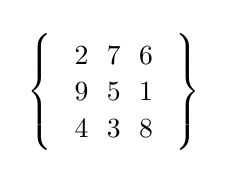
\begin{tikzpicture}
\matrix () [matrix of math nodes, left delimiter = \{, right delimiter = \}]
{%
2 & 7 & 6 \\
9 & 5 & 1 \\
4 & 3 & 8 \\
};
\end{tikzpicture} $$

$$ 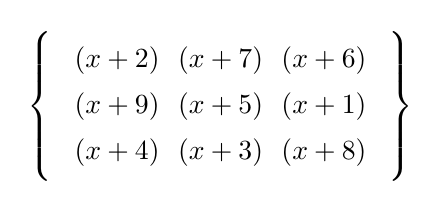
\begin{tikzpicture}
\matrix () [matrix of math nodes, left delimiter = \{, right delimiter = \}]
{%
(x + 2) & (x + 7) & (x + 6) \\
(x + 9) & (x + 5) & (x + 1) \\
(x + 4) & (x + 3) & (x + 8) \\
};
\end{tikzpicture} $$

Calculation on the first and last row of the magic square:

\begin{equation} \begin{aligned} \label{eq:c3x1e}
& (x + 2) * (x + 7) * (x + 6) \\
& (x^2 + 7x + 2x + 14) * (x + 6) \\
& x^3 + 6x^2 + 7x^2 + 42x + 2x^2 + 12x + 14x + 84 \\
& x^3 + 15x^2 + \underline{68x} + 84
\end{aligned} \end{equation}

\begin{equation} \begin{aligned} \label{eq:c3x2e}
& (x + 4) * (x + 3) * (x + 8) \\
& (x^2 + 3x + 4x + 12) * (x + 8) \\
& x^3 + 8x^2 + 3x^2 + 24x + 4x^2 + 32x + 12x + 96 \\
& x^3 + 15x^2 + \underline{68x} + 96
\end{aligned} \end{equation}

Compare \eqref{eq:c3x1e} with \eqref{eq:c3x2e}, coefficients of $x^1$ are shared, beside that of $x^2$'s coefficient, which is the cross sum for the magic square accordingly. Continue with a valid order 4x4 magic square by the same method:

$$ 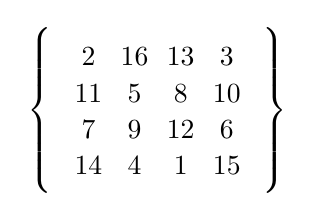
\begin{tikzpicture}
\matrix () [matrix of math nodes, left delimiter = \{, right delimiter = \}]
{%
2 & 16 & 13 & 3 \\
11 & 5 & 8 & 10 \\
7 & 9 & 12 & 6 \\
14 & 4 & 1 & 15 \\
};
\end{tikzpicture} $$

$$ 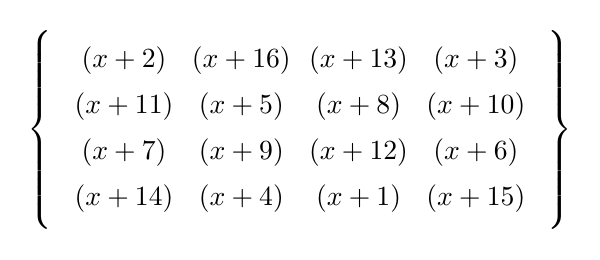
\begin{tikzpicture}
\matrix () [matrix of math nodes, left delimiter = \{, right delimiter = \}]
{%
(x + 2) & (x + 16) & (x + 13) & (x + 3) \\
(x + 11) & (x + 5) & (x + 8) & (x + 10) \\
(x + 7) & (x + 9) & (x + 12) & (x + 6) \\
(x + 14) & (x + 4) & (x + 1) & (x + 15) \\
};
\end{tikzpicture} $$

\begin{equation} \begin{aligned} \label{eq:c4x1e}
& (x + 2) * (x + 16) * (x + 13) * (x + 3) \\
& (x^2 + 16x + 2x + 32) * (x + 13) * (x + 3) \\
& (x^3 + 13x^2 + 16x^2 + 208x + 2x^2 + 26x + 32x + 416) * (x + 3) \\
& x^4 + 3x^3 + 13x^3 + 39x^2 + 16x^3 + 48x^2 + 208x^2 + 624x + 2x^3 + 6x^2 + 26x^2 + 78x + & 32x^2 + 96x + 416x + 1248 \\
& x^4 + 34x^3 + \underline{359x^2} + 1214x + 1248
\end{aligned} \end{equation}

\begin{equation} \begin{aligned} \label{eq:c4x2e}
& (x + 14) * (x + 4) * (x + 1) * (x + 15) \\
& (x^2 + 4x + 14x + 56) * (x + 1) * (x + 15) \\
& (x^3 + 1x^2 + 4x^2 + 4x + 14x^2 + 14x + 56x + 56) * (x + 15) \\
& x^4 + 15x^3 + 1x^3 + 15x^2 + 4x^3 + 60x^2 + 4x^2 + 60x + 14x^3 + 210x^2 + 14x^2 + 210x + & 56x^2 + 840x + 56x + 840 \\
& x^4 + 34x^3 + \underline{359x^2} + 1166x + 840
\end{aligned} \end{equation}

Compare \eqref{eq:c4x1e} and \eqref{eq:c4x2e} , the same coefficient common to both polynomials has $x^2$ instead of $x^1$. The following conclusion is made about the coefficient's position:

\begin{equation*}
x^3 - x^1 = x^4 - x^2 \Rightarrow
x^2 = x^2 \Rightarrow x^{n-2}
\end{equation*}

\begin{equation}
x^{n-2}
\end{equation}

\section{The Property}
Construct a magic square of order 3x3 with cells a, b, c, ... i:

$$ 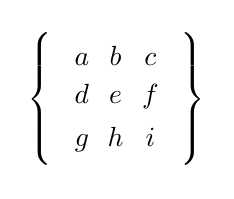
\begin{tikzpicture}
\matrix () [matrix of math nodes, left delimiter = \{, right delimiter = \}]
{%
a & b & c \\
d & e & f \\
g & h & i \\
};
\end{tikzpicture} $$

Take each cell and let it be the root of a polynomial:

$$ 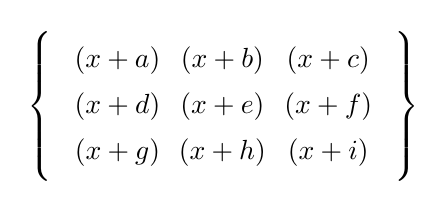
\begin{tikzpicture}
\matrix () [matrix of math nodes, left delimiter = \{, right delimiter = \}]
{%
(x + a) & (x + b) & (x + c) \\
(x + d) & (x + e) & (x + f) \\
(x + g) & (x + h) & (x + i) \\
}; \label{eq:MS}
\end{tikzpicture} $$

Then continue to solve the first row's polynomial and according to \eqref{eq:c3x1e} and \eqref{eq:c3x2e}, choose terms with $x^1$ as the variable to construct a formula:

\begin{equation*} \begin{aligned}
& (x + a) * (x + b) * (x + c) \\
& (x^2 + bx + ax + ab) * (x + c) \\
& x^3 + cx^2 + bx^2 + \underline{bcx} + ax^2 + \underline{acx} + \underline{abx} + abc \\
& bcx + acx + abx \\
& \frac{bcx + acx + abx}{x} \\
& bc + ac + ab = x
\end{aligned} \end{equation*}

\begin{equation}
bc + ac + ab = x \label{eq:ee3x1}
\end{equation}

For clarity and later use in constructing a general formula, factor out c in \eqref{eq:ee3x1}:

\begin{equation} \label{eq:e3x1}
c(b + a) + ab = x
\end{equation}

Continue with the same method for the last row, yielding the result:

\begin{equation} \label{eq:e3x2}
i(h + g) + gh = x
\end{equation}

Now compare \eqref{eq:e3x1} with \eqref{eq:e3x2}, and by \eqref{eq:c3x1e} and \eqref{eq:c3x2e}:

\begin{equation}
c(b + c) + ab = i(h + g) + gh
\end{equation}

Extend this process for the first and last columns respectively:

\begin{equation*} \begin{aligned}
& (x + a) * (x + d) * (x + g) = (x + c) * (x + f) * (x + i) \\
& g(d + a) + ad = i(f + c) + cf
\end{aligned} \end{equation*}
\begin{equation*} \begin{aligned}
& 4(9 + 2) + (9)(2) = 8(1 + 6) + (6)(1) \\
& 4(11) + 18 = 8(7) + 6 \\
& 44 + 18 = 56 + 6 \\
& 62 = 62
\end{aligned} \end{equation*}

\begin{equation}
g(d + a) + ad = i(f + c) + cf
\end{equation}

In order to carry out the same calculations on the center row or column of a magic square, a row and a column has to be used instead:

\begin{equation*} \begin{aligned}
& (x + b) * (x + e) * (x + h) = (x + d) * (x + e) * (x + f) \\
& h(e + b) + be = f(e + d) + de
\end{aligned} \end{equation*}

\begin{equation*} \begin{aligned}
& 3(5 + 7) + (7)(5) = 1(5 + 9) + (9)(5) \\
& 3(12) + 35 = 1(14) + 45 \\
& 36 + 35 = 14 + 45 \\
& 71 = 59
\end{aligned} \end{equation*}

\begin{equation}
h(e + b) + be \not = f(e + d) + de
\end{equation}

Examine the two diagonals:

\begin{equation*} \begin{aligned}
& (x + a) * (x + e) * (x + i) = (x + c) * (x + e) * (x + g) \\
& i(e + a) + ae = g(e + c) + ce
\end{aligned} \end{equation*}

\begin{equation*} \begin{aligned}
& 8(5 + 2) + (2)(5) = 4(5 + 6) + (6)(5) \\
& 8(7) + 10 = 4(11) + 30 \\
& 56 + 10 = 44 + 30 \\
& 66 = 74
\end{aligned} \end{equation*}

\begin{equation}
i(e + a) + ae \not = g(e + c) + ce
\end{equation}

Notice, the results of calculation on a center row and column are not equal to one another as well as calculations on the two diagonals.

\subsection{Order 3x3 and Beyond}
The formula for a magic square of order 4x4 is as follows by calculation \eqref{eq:c4x1e} and \eqref{eq:c4x2e}:

\begin{equation*} \begin{aligned}
& (x + a) * (x + b) * (x + c) * (x + d) \\
& (x^2 + bx + ax + ab) * (x + c) * (x + d) \\
& (x^3 + cx^2 + bx^2 + bcx + ax^2 + acx + abx + abc) * (x + d) \\
& x^4 + dx^3 + cx^3 + \underline{cdx^2} + bx^3 + \underline{bdx^2} + \underline{bcx^2} + bcdx + \\ & ax^3 + \underline{adx^2} + \underline{acx^2} + acdx + \underline{abx^2} + abdx + abcx + abcd \\
& cdx^2 + bdx^2 + bcx^2 + adx^2 + acx^2 + abx^2 \\
& \frac{cdx^2 + bdx^2 + bcx^2 + adx^2 + acx^2 + abx^2}{x^2} \\
& cd + bd + bc + ad + ac + ab = x
\end{aligned} \end{equation*}

\begin{equation}
cd + bd + bc + ad + ac + ab = x \label{eq:ee4x1}
\end{equation}

Factor out c to match equation \eqref{eq:e3x1} and then factor d accordingly:

\begin{equation} \label{eq:e4x1}
d(c + b + a) + c(b + a) + ab = x
\end{equation}

whereby \eqref{eq:e3x1} and \eqref{eq:e4x1}, it follows for a magic square of order 5x5 that:

\begin{equation}
c(b + a) + ab = x \Rightarrow d(c + b + a) + c(b + a) + ab = x \Rightarrow e(d + c + b + a) + d(c + b + a) + c(b + a) + ab = x \label{eq:q5x1}
\end{equation}

And by calculation:

\begin{equation*} \begin{aligned}
& (x + a) * (x + b) * (x + c) * (x + d) * (x + e) \\
& (x^2 + bx + ax + ab) * (x + c) * (x + d) * (x + e) \\
& (x^3 + cx^2 + bx^2 + bcx + ax^2 + acx + abx + abc) * (x + d) * (x + e) \\
& (x^4 + dx^3 + cx^3 + cdx^2 + bx^3 + bdx^2 + bcx^2 + bcdx + ax^3 + adx^2 \\  & + acx^2 + acdx +  abx^2 + abdx + abcx + abcd) * (x + e) \\
& x^5 + ex^4 + dx^4 + \underline{dex^3} + cx^4 + \underline{cex^3} + \underline{cdx^3} + cdex^2 \\ & + bx^4 + \underline{bex^3} + \underline{bdx^3} + bdex^2 + \underline{bcx^3} + bcex^2 + \\ & bcdx^2  + bcdex + ax^4 + \underline{aex^3} + \underline{adx^3} + adex^2 + \underline{acx^3} + \\ & acex^2 + acdx^2 + acdex + \underline{abx^3} + abex^2 + abdx^2 + abdex + abcx^2 + abcex + abcdx + abcde \\
& \frac{dex^3 + cex^3 + cdx^3 + bex^3 + bdx^3 + bcx^3 + aex^3 + adx^3 + acx^3 + abx^3}{x^3} \\
& de + ce + cd + be + bd + bc + ae + ad + ac + ab = x
\end{aligned} \end{equation*}

\begin{equation}
de + ce + cd + be + bd + bc + ae + ad + ac + ab = x \label{eq:ee5x1}
\end{equation}

Factor out c and d, matching equations \eqref{eq:e3x1} and \eqref{eq:e4x1}, then factor out e:

\begin{equation}
e(d + c + b + a) + d(c + b + a) + c(b + a) + ab = x \label{eq:e5x1}
\end{equation}

Which \eqref{eq:e5x1} proves the statement of \eqref{eq:q5x1}.  From \eqref{eq:q5x1}, the pattern is observed, that each preceding term multiplied by all the terms before it, summed together forms a term itself, when added consecutively until the order of the magic square is reached, forms the coefficient for that magic square's order:

\begin{equation}
x_n = n_{k}(n_{k-1} + ... + n_{0}) + ... + n_{k-1}(n_{k-2} + ... + n_{0}) + n_{0}n_{1} \label{eq:fx1}
\end{equation}

And \eqref{eq:fx1} can be Converted to a closed form:

\begin{equation}
x_n = \sum_{k=1}^{n} {n_k(\sum_{j=0}^{k-1} {n_j})} \label{eq:cfx1}
\end{equation}

\subsection{Commutativity of the General formula}
Let the closed form \eqref{eq:cfx1} be separated into the first sum function's summands and for each summand rearrange the variables, factoring out when necessary to prove they are equal forms. This will be done from the second to the fourth summand:

\begin{equation}
ba \Rightarrow ab \label{eq:fs2e}
\end{equation}

\begin{equation} \begin{aligned}
& c(b + a) + ab = b(c + a) + ac = a(c + b) + bc \Rightarrow \\
& cb + ca + ab = cb + ab + ca = ac + ab + cb \label{eq:fs3e}
\end{aligned} \end{equation}

\begin{equation} \begin{aligned}
& d(c + b + a) = c(d + b + a) = b(c + d + a) = a(c + b + d) \not \Rightarrow \\
& dc + db + da = \underline{dc + cb + ca} = \underline{cb + db + ba} = \underline{ca + ba + da} \label{eq:fs4e}
\end{aligned} \end{equation}

At the fourth summand the pattern stops, however each term in \eqref{eq:fs3e} is equivalent to almost every term in \eqref{eq:fs4e}:

\begin{equation*} \begin{aligned}
& \underline{cb} + \underline{ca} + \underline{ab} = \underline{cb} + \underline{ab} + \underline{ca} = \underline{ac} + \underline{ab} + \underline{cb} \Rightarrow \\
& dc + db + da = dc + \underline{cb} + \underline{ca} = \underline{cb} + db + \underline{ba}  = \underline{ca} + \underline{ba} + da
\end{aligned} \end{equation*}

Combine the two summands with a sum and rearrange the variables as before:

\begin{equation*} \begin{aligned}
& d(c + b + a) + c(b + a) = c(d + b + a) + d(b + a) = b(c + d + a) + c(d + a) = a(c + b + d) + c(b + d) \Rightarrow \\
& \underline{dc + db + da + cb + ca} = \underline{dc + cb + ca + db + da} = \underline{cb + dc} + ba + \underline{dc + ca} = \underline{ca} + ba + \underline{da + cb + dc}
\end{aligned} \end{equation*}

Notice all terms are listed except that of ab, which is the preceding summand \eqref{eq:fs2e} of the two sumands, \eqref{eq:fs3e} and \eqref{eq:fs4e}. Thus if all sumands up to n are summed accordingly, then the formula is communicative such that the order of the variables doesn't matter.

\subsection{Examples of the General formula on Invalid Magic Squares}
Let a magic square of order 3x3 have a repetition of a cell's value, calculating the row, column, or diagonal with the repeating cell and the row, column, or diagonal opposite of it, using \eqref{eq:e3x1}:

$$ 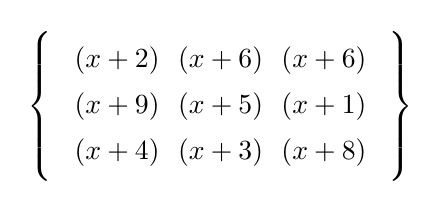
\begin{tikzpicture}
\matrix () [matrix of math nodes, left delimiter = \{, right delimiter = \}]
{%
(x + 2) & (x + 6) & (x + 6) \\
(x + 9) & (x + 5) & (x + 1) \\
(x + 4) & (x + 3) & (x + 8) \\
};
\end{tikzpicture} $$

\begin{equation*} \begin{aligned}
& 6(6 + 2) + (2)(6) = 8(3 + 4) + (4)(3) \\
& 6(8) + 12 = 8(7) + 12 \\
& 48 + 12 = 56 + 12 \\
& 60 = 68
\end{aligned} \end{equation*}

Let a magic square of order 3x3 have a new cell value, such that the cross sums do not match, using the same method as before to check it:

$$ 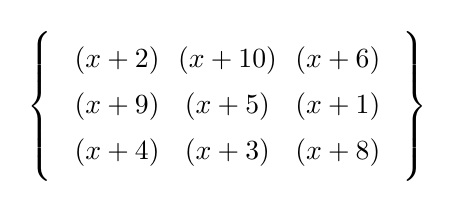
\begin{tikzpicture}
\matrix () [matrix of math nodes, left delimiter = \{, right delimiter = \}]
{%
(x + 2) & (x + 10) & (x + 6) \\
(x + 9) & (x + 5) & (x + 1) \\
(x + 4) & (x + 3) & (x + 8) \\
};
\end{tikzpicture} $$

\begin{equation*} \begin{aligned}
& 6(10 + 2) + (2)(10) = 8(3 + 4) + (4)(3) \\
& 6(12) + 20 = 8(7) + 12 \\
& 72 + 20 = 56 + 12 \\
& 92 = 68
\end{aligned} \end{equation*}

Let a magic square have both a repeating cell value and a mismatching cross sum and continue by the same process:

$$ 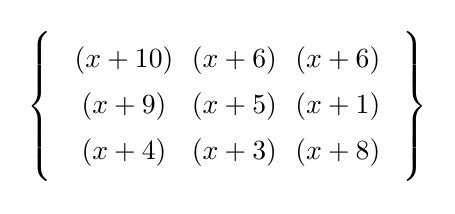
\begin{tikzpicture}
\matrix () [matrix of math nodes, left delimiter = \{, right delimiter = \}]
{%
(x + 10) & (x + 6) & (x + 6) \\
(x + 9) & (x + 5) & (x + 1) \\
(x + 4) & (x + 3) & (x + 8) \\
};
\end{tikzpicture} $$

\begin{equation*} \begin{aligned}
& 6(6 + 10) + (10)(6) = 8(3 + 4) + (4)(3) \\
& 6(16) + 60 = 8(7) + 12 \\
& 96 + 20 = 56 + 12 \\
& 116 = 68
\end{aligned} \end{equation*}

Thus if a magic square is invalid, then the equation does not hold true. Contrary to this, by \eqref{eq:c3x1e} and \eqref{eq:c3x2e}, a magic square that does not have repeating cell values or mismatching cross sums the equations holds true. Thus in order for a magic square to be valid it must adhere to \eqref{eq:e3x1} for both the first and last rows as well as the first and last columns:

\begin{equation}
c_0(b_0 + a_0) + a_0b_0 = c_1(b_1 + a_1) + a_1b_1 \label{eq:cs3x1}
\end{equation}

It follows that for a magic square to be squared, not just all cross sums should match and have no repeating cells, but also follow the equality of the formula:

\begin{equation}
c^2_0(b^2_0 + a^2_0) + a^2_0b^2_0 = c^2_1(b^2_1 + a^2_1) + a^2_1b^2_1 \label{eq:cs3x2}
\end{equation}

Apply this to a well known squared magic square, namely The Parker Square, which includes both repeating cell values and a mismatching cross sum:

$$ 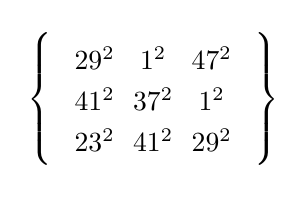
\begin{tikzpicture}
\matrix () [matrix of math nodes, left delimiter = \{, right delimiter = \}]
{%
29^2 & 1^2 & 47^2 \\
41^2 & 37^2 & 1^2 \\
23^2 & 41^2 & 29^2 \\
};
\end{tikzpicture} $$

$$ 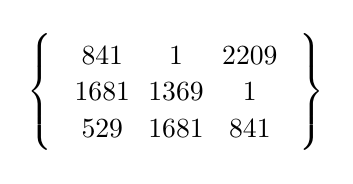
\begin{tikzpicture}
\matrix () [matrix of math nodes, left delimiter = \{, right delimiter = \}]
{%
841 & 1 & 2209 \\
1681 & 1369 & 1 \\
529 & 1681 & 841 \\
};
\end{tikzpicture} $$

\begin{equation*} \begin{aligned}
& 2209(1 + 841) + (841)(1) = 841(1681 + 529) + (529)(1681) \\
& 2209(842) + 841 = 841(2210) + 889249 \\
& 1859978 + 841 = 1858610 + 889249 \\
& 1860819 = 2747859
\end{aligned} \end{equation*}

It can be seen at once that the attempt does not satisfy the formula of \eqref{eq:cs3x2}.

\section{Remarks}
This property of magic squares is of use to minimize computation for the search of a squared magic square by reducing the problem to the question of whether two triplets of values exist such that they satisfy the formula of \eqref{eq:cs3x2}. Subsequent values can be found by the use of the same formula, where at least two variables will already be known, further reducing computation. The center cell, which is only present for odd magic squares can be found by just counting up the cell's value from 1.

For the entirety of this paper, the letters a-z were used as it was a clearer representation, but for formulas like \eqref{eq:cs3x1} and \eqref{eq:cs3x2}, this is not ideal as it implies a row, column, or diagonal from previous notation given for a magic square, instead the usual notation of $x_n$ is better.

What is now needed for computation, using the formulas as just described with the usual notation of $x_n$:
\begin{equation}
x^2_3(x^2_2 + x^2_1) + x^2_1x^2_2 = x^2_6(x^2_5 + x^2_4) + x^2_4x^2_5
\end{equation}


\begin{equation}
x^2_3(x^2_7 + x^2_1) + x^2_1x^2_7 = x^2_6(x^2_8 + x^2_4) + x^2_4x^2_8
\end{equation}

\begin{equation}
x^2_9
\end{equation}

The preceding equations are only for a magic square of order 3x3 respectively.

Take note that the formula of \eqref{eq:cs3x1} is the same as \eqref{eq:cs3x2}, just with larger values. This can be shown by squaring the variables of the order 3x3 magic square seen in \autoref{eq:MS}:

$$ 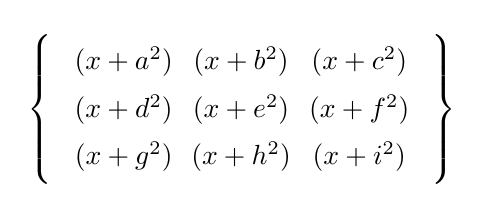
\begin{tikzpicture}
\matrix () [matrix of math nodes, left delimiter = \{, right delimiter = \}]
{%
(x + a^2) & (x + b^2) & (x + c^2) \\
(x + d^2) & (x + e^2) & (x + f^2) \\
(x + g^2) & (x + h^2) & (x + i^2) \\
};
\end{tikzpicture} $$

\begin{equation*} \begin{aligned}
& (x + a^2) * (x + b^2) * (x + c^2) \\
& (x^2 + b^2x + a^2x + a^2b) * (x + c^2) \\
& x^3 + c^2x^2 + b^2x^2 + \underline{b^2c^2x} + a^2x^2 + \underline{a^2c^2x} + \underline{a^2b^2x} + a^2b^2c^2 \\
& b^2c^2x + a^2c^2x + a^2b^2x \\
& \frac{b^2c^2x + a^2c^2x + a^2b^2x}{x} \\
& b^2c^2 + a^2c^2 + a^2b^2 = x
\end{aligned} \end{equation*}

\begin{equation}
b^2c^2 + a^2c^2 + a^2b^2 = x \label{eq:ee3x3}
\end{equation}

Factor out $c^2$ to achieve the form of \eqref{eq:cs3x2}:

\begin{equation}
c^2(b^2 + a^2) + a^2b^2 = x \label{eq:e3x3}
\end{equation} \\

About the closed form, when imputed into Desmos it produces the series A019582 ($a(n) = n*(n - 1)^3/2$) from the OEIS. The exact form used for this observation:

\begin{equation}
x=\sum_{k=1}^{n}n\left(\sum_{j=0}^{k-1}n\right)
\end{equation} \\

Definitions were purposely not given as i couldn't find satisfactory descriptions, for rearranging a variable and what it means for a magic square to be valid. For the former definition, to rearrange variables is to swab the current value of some variable with an other variable's value and vice versa. As for the ladder, a valid magic square being non-parker is very much sufficient. \\

A back burner problem can be quite useful in the search for knowledge in mathematics, subverting all reason as a problem so seemingly useless sums with the whole of mathematics in a beneficial way.

\end{document}